\vspace*{4pt}
\section{Study}
\label{sec:study}

In this study, we investigate whether the use of a recommender system 
can improve the effectiveness of test case prioritization techniques.
We consider the following research questions.

\begin{smallitem}
\item[RQ1:] Can our recommender system be useful for 
improving the effectiveness of test case prioritization techniques?

\item[RQ2:] Can we improve the fault detection rate when we have
only limited budget of time to test the entire system? 
\end{smallitem}

The following subsections present our objects of analysis, 
study setup, threats to validity, and data analysis.

\vspace*{4pt}
\subsection{Objects of Analysis}
\label{sec:objects}

To investigate our research questions, we performed an empirical study 
using two open source applications and one commercial web application.

\textbf{DASCP} is a digital archive and scan software for civil projects; 
 we obtained this application from a private company.  
DASCP is a web based application designed to store civil project 
contracts, which include the technical information of civil and construction projects 
such as project plans and relevant associated information. 
DASCP includes an access control system and provides two types of access rights: 
one user group has permission to edit or insert a project's information or 
upload maps and contract sheets. The other user group is only allowed to view 
the data and details about the projects.

Our second application is \textbf{nopCommerce}, which is a widely-used open 
source e-commerce shopping cart web application with more than 1.8 million 
downloads. This application is written in ASP.Net MVC and uses 
Microsoft SQL Server as a database system ~\cite{nopCommerece}. 

Our last application is \textbf{Coevery}, which is an open source 
customer relationship management (CRM) system written in ASP.Net. 
This application provides an easy framework for users to create their own customized 
modules without having to write any code. The UI design of Coevery has been developed 
by AngularJS and Orchard Technologies~\cite{coevery}. 

\begin{table}
\caption{Subject Applications Properties}
\begin{center}
\begin{tabular}{|l|c|c|c|} \hline
\textbf{Metrics}  & \textbf{DASCP} & \textbf{nopCommerce} 
& \textbf{Coevery} \\\hline \hline
Classes   & 107  & 1,919& 2,258 \\\hline
Files  & 201  & 1,473 & 1,875 \\\hline
Functions & 940  & 21,057 & 13,041 \\\hline
LOC & 35,122 & 226,354 &120,897 \\\hline
Sessions  & 748 & 1310 & 274 \\\hline
Faults  & 35 & 70 & 30\\\hline
Version  & 3 & 23 & 3 \\\hline
Test Cases & 95& 543 & 1,120 \\\hline
Installations & 3 & 2 & 1 \\\hline
\end{tabular}
\end {center}
\label{tab:AUTs}
\end{table}

Table~\ref{tab:AUTs} lists the applications under study and
their associated data: ``Classes'' (the number of class files), 
``Files'' (the number of files), ``Functions'' (the number of 
functions/methods), ``LOC'' (the number of lines of code), 
``Sessions'' (the number of user sessions that we collected), 
``Faults'' (the number of seeded faults), ``Version'' (the number 
of versions), ``Test Cases'' (the number of test cases), and
``Installations'' (the number of different locations where the 
applications were installed). 

Test cases were in application package and we did not implement any 
new test case. Version of open source applications were downloaded 
form the applications' \textit{GitHub} repository and we downloaded all available versions. 


\vspace*{4pt}
\subsection{Variables and Measures}
\label{sec:measures}

\subsubsection{Independent Variable}

To investigate our research questions, we manipulated one independent 
variable: prioritization technique. 
We considered five different test case prioritization techniques,
which we classified into two groups: control and heuristic.
Table~\ref{tab:techniques} summarizes these groups and techniques.
The second column shows prioritization techniques for each group, 
and the third column is a short description of prioritization techniques. 

\begin{table*}[!ht]
\caption{Test Case Prioritization Techniques}
\vspace*{-10pt}
\begin{center}
\begin{tabular}{|l|l|l|}\hline
Group & Technique & Description \\ \hline
\multirow{4}{*}{Control} 
& Change history-based ($T_{ch}$) & Test case prioritization based on change impact analysis score.\\
& Most frequent web forms-based ($T_{mfw}$)&  Test case prioritization based on value of frequency for each web form.\\
& Most frequent methods-based ($T_{mfm}$) &  Test case prioritization based on value of frequency for each method.\\
& Random ($T_{r}$) &  Test execution in random order.\\	
& Greedy ($T_{g}$) &  Test case prioritization in based on code coverage.\\\hline			
\multirow{2}{*}{Heuristic} 
& Hybrid collaborative filtering-based ($T_{hcf}$)& Test case prioritization based on the proposed technique. \\
& Reverse Hybrid collaborative filtering-based ($T_{hcfr}$)& Test case prioritization based on the proposed technique with descending ranking values. \\\hline
\end{tabular}
\end {center}
\label{tab:techniques}
\vspace*{-5pt}
\end{table*}

As shown in Table~\ref{tab:techniques}, we considered four control techniques and 
one heuristic technique. For our heuristic technique, we used the approach 
explained in Section~\ref{sec:approach},
so, here, we only explain the control techniques we applied as follows:

%\vspace*{-5pt}
\subsubsection*{Change History-Based ($T_{ch}$)}
The first control technique is test case prioritization based on change impact
score. In order to perform this technique, we used the information that
we obtained from the change impact analysis approach, which we explained in 
Section ~\ref{CIA-approach}. We prioritized our test cases based on the 
highest scores of the change impact matrix. 
	
%\vspace*{-5pt}
\subsubsection*{Most Frequent Web Forms-Based ($T_{mfw}$)}
This approach determines the web forms that have been most frequently used by users. 
We assume that the most frequently used web forms play a more important role in the system; 
eventually, they should have a higher priority to be tested first. Another reason
why the frequency of web pages is the key for testing is that the most frequently used web pages usually 
contain more functionality and links with other pages, so any bugs on 
those pages can affect greater portion of the entire system. 
Here we define ``base session'' as a long session conducted by our users 
that displays the most interactions in the application.
We picked 20\% of our total sessions as base sessions. 
For example, in online shopping, our base session is a sequence of actions
from user login to checkout, including all necessary actions and some 
random unnecessary actions such as browsing for other items, 
checking the inbox during the shopping process, etc. 
	
\begin{figure}[!ht]
	\centering
	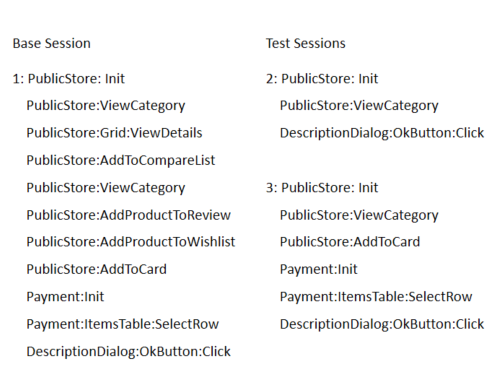
\includegraphics[width=0.90\linewidth]{./SessionSample2.png}
	\vspace*{3pt}
	\caption{Sample of Base Session and Test Sessions}
	\label{fig:sessions}
\vspace*{5pt}
\end{figure}
	
After collecting all sessions, we conducted an analysis of web pages frequency 
by comparing the observed web forms in each session with a base session. 
	
\[
{F_{w,i} = \frac {\sum_{{page\: score\: for \: each\: session}}(S_{i})}
	{\sum_{{number \: of \: base \: sessions}}({BS_{i}})}}	
\]
	
Using Figure ~\ref{fig:sessions} as an example, the page ``PublicStore'' from the base session 
was observed in test sessions 2 and 3. If we assume that we have 
ten test sessions and three base sessions,
and this particular page was observed in seven of the ten pages, then the
frequency of page ``PublicStore'' is equal to $(0.7 / 3) = 0.23$
	
%\vspace*{-5pt}
\subsubsection*{Most Frequent Methods-Based ($T_{mfm}$)}
The most frequent methods approach is nearly identical to the web form frequency technique. 
The only difference is that we considered a method instead of a web form 
as a comparison factor. 
The most frequent methods, usually have high dependency on the other classes and methods. 
If one of them fails, it can cause a significant failure or degradation of the system. 
In order to prevent a domino effect in the system, high frequency methods 
should be tested first, because their failure can cause 
other components failure due to their dependencies.	 	
%Heuristic technique in this study is permuting test cases 
%based on the output list of our	recommender system. 

%\vspace*{-5pt}
\subsubsection*{Random ($T_{r}$)}

Random prioritization selects a test cases in random order.
In this control technique, we randomly selected test cases until
we had executed 100\% of the test cases. \\
	
\subsubsection{Dependent Variable} 

Our dependent variable RQ1 is the average percentage of fault detection (APFD)
referring to the average percentage of faults detected during the test suite execution. 
The range of APFD is from 0 to 100, the higher value indicating better prioritization technique. 
Given $T$ as a test suite with $n$ test cases and $m$ number of faults, 
$F$ as a collection of detected faults by $T$ and
$TF_{i}$ as the first test case that catches the fault $i$, 
we calculate APFD ~\cite{apfd} as follows:

\[
{APFD = 1- \frac {{TF_{1} + TF_{2} + ... + TF_{m}}} {nm} + \frac{1}{2n}}
\]
	
RQ2 seeks to measure the effectiveness of our proposed approach
when we have constrained resources, which means that we need to evaluate 
the effectiveness of our approach using a different metric. 
Qu et al.~\cite{myra} defined the normalized metric of APFD, which is the
area under the curve when the numbers of test cases or faults are not consistent. 
The NAPFD formula is as follows:
	
\[
{NAPFD = p- \frac {{TF_{1} + TF_{2} + ... + TF_{m}}} {nm} + \frac{p}{2n}}
\]
	
In this formula, $n$ is percentage of the test suite run, 
$m$ represents the total number of faults found by all test cases,
$TF_{i}$ indicates the same parameter as AFPF, and 
$p$ is the number of faults detected by percentage of our
budget divided by total number of detected faults when 
running 100\% of test cases.  
	
\subsection{Data Collection and Experimental Setup}
\label{data-collection}
In order to perform our experiment, for both the control and heuristic techniques
we needed to collect three different types of datasets: telemetry data, change 
history, and code coverage information. We explain the data collection processes
in the following subsections.

\subsubsection{Collection of Telemetry Data}
To collect telemetry data, we implemented a small function to record user interactions. 
We considered a sequence of each user's interactions on a specific date as a user session.
First, we uploaded two applications, {\em Coevery} and {\em nopCommerce}, on IIS server 
at the University of ABC in November 2016. 
The server specification is CPU Core i7 with 16 GB of RAM.
After deploying our applications, we recruited volunteer graduate and undergraduate
computer science students and assigned a variety of tasks to them. 
Assigned task to the volunteers were simple scenarios that each application is designed for.
For example, in {\em nopCommerce} we asked them to perform online shopping 
by taking the actual steps which starts from login to payment. We also asked some of 
the users to be the system administrator so we could monitor the whole system 
rather than only the end user side.
We also asked the end users to check the other part of the system randomly like
checking their inbox or wish-list.  
In total, seventy volunteer students performed different tasks during a 40 days period.  
%%% revierw question
In total we collected 1310 and 274 user sessions for {\em nopCommerce} 
and {\em Coevery} respectively. 
%%%%
 
The data collection process for {\em DASCP} is different from that of {\em Coevery} 
and {\em nopCommerce}. {\em DASCP} is a commercial and closed source application 
that has three versions, and it has been installed on the servers of three companies since 2011. 
The DASCP users whose data we examined are real users, and they have application domain knowledge.
We collected twelve-months period of user interactions for DASCP.
As described in Section~\ref{sec:objects}, DASCP provides two types of access rights for users.
In this study, we only considered the sessions of those users who have full access to the system.
In total, 748 user sessions were collected during that period of time. 

%%% more details about sessions
However, the length of the sessions varied by user, date and and workplace.
For example, some users performed all their assigned task few hours before the
determined deadline, while others distributed their tasks into several days.
Average length of user session for {\em nopCommerce} is equal to 56 and for
{\em Coevery} is 24. Although, in some case we obtained sessions length over 
300, specially when the interaction date was close to the deadline. 
Also, most of the {\em Coevery} users are selected from graduate students since the
functionality of this application is relatively more complex than {\em nopCommerce}. 

Figure ~\ref{fig:SampleSession3} shows an example of the raw telemetry data. 
The left column shows the session identifier, which is a user
navigating through the system. The right column is the set of server side user interactions. The structure of the interactions is of the format (Form name):(Control name):(Action name).

\begin{figure}[!ht]
	\centering
	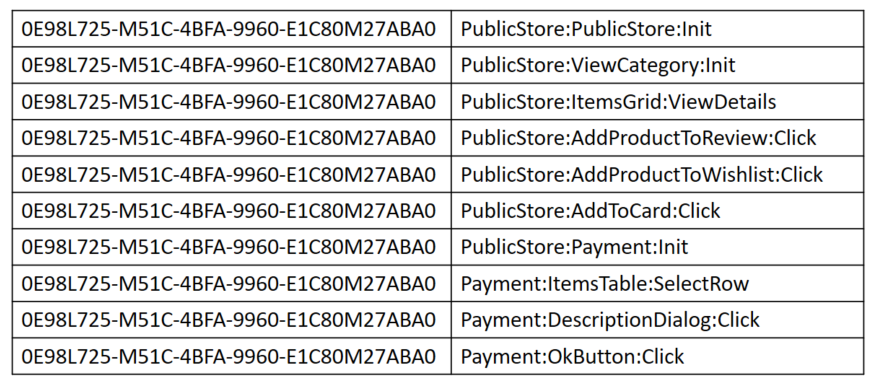
\includegraphics[width=0.90\linewidth]{./SessionSample3.png}
	\vspace*{3pt}
	\caption{Sample User Session}
	\label{fig:SampleSession3}
	\vspace*{5pt}
\end{figure}


\subsubsection{Collection of Code Change History}
We had to take three steps to measure change impact. 
First, we needed a clear understanding of the applications with respect to their changes.
For instance, we needed to check whether a change 
was just the renaming a variable or component, the addition of some comments, 
or an alternation of code by adding or deleting functions, and so on. 
Then, we needed to check whether changes had been made in the current version, 
and finally, we tested a recently changed system~\cite{change3}. 
In order to collect change history information for training, 
we used all versions of our applications.

In our study, we collected the change history of our three applications. 
We chose ten metrics that have high correlations with bugs.
Most of these metrics have been used in bug detection research, and they
are known to be good indicators for locating bugs~\cite{sungmicro, shihab12, 
raimund, change1, change2}.
Table~\ref{tab:historyMetrics} shows the applied change metrics in this study. 

\begin{table}[!ht]
\caption{Change metrics used to evaluate risk in this study}	
\vspace*{3pt}
%\begin{tabular*} {.8\linewidth}{@{\extracolsep{\fill}}l|l|}
\begin{tabular} {|l|l|} \hline
	\textbf{Metrics Name} & \textbf{Description} \\\hline \hline
	Revision & Number of revision of a component  \\\hline
	LOC Added&   Added lines of code \\\hline
	Max LOC Added  & Maximum added lines of code \\\hline
	AVE LOC Added  & Average added lines of code \\\hline
	LOC Deleted  & Deleted lines of code  \\\hline
	Max LOC Deleted & Maximum deleted line\\\hline
	AVE LOC Deleted & Average deleted lines of code \\\hline
	Code Churn & Sum of change in all revisions \\\hline
	Max Code Churn & Maximum code churn for all revisions \\\hline
	AVE Code Churn & Average code churn per revisions \\\hline
	Age & \parbox[t]{5cm}{Age of a component \\ in days from last release} \\\hline
	Time & \parbox[t]{5cm} {Time of a change \\ in dd-mm-yyyy format} \\\hline		
\end{tabular}
\label{tab:historyMetrics}
\end{table}

\subsubsection{Collect Code Coverage}
\label{codecoverage}
Once our recommender system was designed and implemented, 
we needed to find test cases that covered the recommended components. 
We collected the code coverage data for our test cases using code coverage analysis tool  
that Microsoft Visual Studio provides as part of its framework. 
After collecting the code coverage information, 
we entered that information into a relational database. We assigned unique
identifier values for each method and test case which provides
a key for method and test tables. So we could easily map the methods
to the test cases that exercise them.  

 
\begin{table}[!ht]
\caption{Code Coverage Data Table}
%\vspace*{-10pt}
\begin{center}
\begin{tabular}{|c|c|c|c|c|c|} \hline
	MethodID  & Risk Score & TestID1 & ... & TestID n \\\hline
	12 & 0.876 & 0 &  & 0 \\\hline
	287 & 0.012 & 1 &  & 0 \\\hline
	301 & 0.547 & 0 &  & 0 \\\hline
	148 & 0.145 & 0 &  & 1 \\\hline
	67 & 0.055 & 1 &  & 0 \\\hline			
\end{tabular}
\end {center}
\label{tab:coverage}
%\vspace*{-15pt}
\end{table}

	
Table~\ref{tab:coverage} show the code coverage data we collected.
%In our database system these columns are in separate tables and we join them
%by module identifier but to save the space here, we represent them as one table.   
The first column, ``MethodID'', shows
the unique identifier values that we assigned for each method. 
The second column shows the final risk scores, which is the output of 
our recommender system. Other columns list our test cases
with Boolean values: 0 indicates that the test case does not cover 
the method, and 1 indicates that the test case covers the method.

\subsubsection{Seeded Faults}
\label{faultsInfo}
As mentioned in ~\ref{}, faults were seeded manually by graduate students. 
We tried to simulate the naturally developer faults into the applications. 
All seeded faults are in server-side code level and we ignored HTML-based and GUI faults. 
Four types of faults were seeded into the applications. 
First type is data faults, which are faults that related to the interacting with the data store. 
Logic faults that are logic error in code, action faults that modifies parameter values and actions, 
and finally, linkage faults that change the hyperlinks references.  



Once the change history data is collected, we applied 
ANOVA analysis to our dataset to obtain a linear model.
Our goal was to find the correlation coefficient for each 
metric to measure statistical relationships between 
a variable and real defects. The value of this measure 
fluctuates between 1 and -1, where 1 indicates a strong 
positive relationship, 0 indicates no correlation, and 
negative value means reverse correlation.
For example, if we have a -0.87 correlation coefficient score for 
$Age$ metric that indicates that the oldest components of the system
has a less risk of regression faults.   
We also calculated root mean squared error and mean absolute error. 
A lower error value shows that the model has higher prediction accuracy. 
 

In order to evaluate our linear model, we applied 10-fold cross validation. 
By applying linear regression, we obtained a model that determines the weight 
of each variable. In next step we applied our obtained model  
to evaluate the risk score of each component. 
Finally, by having a matrix of components and their relevant risk scores, 
we permuted the test cases. For example, suppose we have five components
$C =\{c_1, c_2, ... , c_5\}$ with risk score 
as follows :   $R =\{0.0014, 0.251, 0.034 , 0.561, 0.138\}$.
Also, suppose we have a list of test cases with their code coverage information.
Then, we will reorder the test cases in such a way to test $c_4$ first, 
since it has highest risk score (0.561), and $c_1$ will be the last 
component to be tested. 

After collecting all the required data, we ran control and heuristic 
techniques and calculated APFD and NAPFD values for the reordered test cases 
to determine whether the proposed technique improved the fault detection rate. 

